\documentclass[]{beamer}

% beamer options
	%\setbeamercovered{transparent}
% custom commands
	\def\colorize<#1>{%
\temporal<#1>{\color{red!50}}{\color{black}}{\color{black!50}}}

\usepackage{tikz}
\usetikzlibrary{arrows, shapes.geometric, backgrounds}
\usepackage{minted}

\author{Tejas Sanap}
\title{Introduction to \LaTeX}
\date{December 28, 2019}

\begin{document}
	\begin{frame}
		\titlepage
	\end{frame}

	\begin{frame}[fragile,t]
		\frametitle{How do we write a document?}
			The process of creating a document comprises of two components:
			\onslide<2->{
				\begin{itemize}
					\item Deciding \textbf{what} the content \textbf{should be}\ldots
					\item Deciding \textbf{how} the content \textbf{should look}\ldots
				\end{itemize}
			}
					\def\cirA{(0,0) circle (2cm)}
					\def\cirB{(3,0) circle (2cm)}
					\colorlet{circle edge}{red!50}
					\colorlet{circle area}{red!20}
					\tikzset{
						filled/.style={fill=circle area, draw=circle edge, thick},
						outline/.style={draw=circle edge, thick},
						filled1/.style={fill=blue!20, draw=blue!50, thick},
						outline1/.style={draw=blue!50, thick},
						filled2/.style={fill=green!20, draw=green!50, thick},
						outline2/.style={draw=green!50, thick},
					}
			\only<3>{
				\begin{figure}
					\centering
					\begin{tikzpicture}
						\begin{scope}
							\clip \cirA;
							\draw[filled2] \cirB;
						\end{scope}
						\draw[outline2] \cirA node {Matter};
						\draw[outline2] \cirB node {Form};
					\end{tikzpicture}
				\end{figure}
			}
			\only<4>{
				\begin{figure}
					\centering
					\begin{tikzpicture}
						\begin{scope}
							\clip \cirB;
							\draw[filled, even odd rule] \cirA 
														 \cirB node {Form};
						\end{scope}
						\begin{scope}
							\clip \cirA;
							\draw[filled1, even odd rule] \cirB
														  \cirA node {Matter};
						\end{scope}
						\draw[outline1] \cirA;
						\draw[outline] \cirB;
					\end{tikzpicture}
				\end{figure}
			}
	\end{frame}

	\begin{frame}[t]
		\frametitle{Type-setting?}
		\onslide<1->{What is type-setting?}

		\onslide<2->{
		\begin{itemize}
			\item The process of arranging the various objects on a page.
			\item It is process that takes place after the manuscript has been written.
		\end{itemize}
		}
		\onslide<3-4>{
			How \only<3>{do}\only<4>{should} we typeset? \\
			\only<3>{\Huge{MS WORD!}}
			\only<4>{\Huge{{\LaTeX}!}}
		}
		\onslide<5>{
			Unlike WYSIWYG softwares like MS Word and Open Office, {\LaTeX} seperates the process of typesetting from the process of inserting content.
		}
	\end{frame}

	\begin{frame}
		\frametitle{So, what exactly is {\LaTeX}?}
		\begin{itemize}[<+->]
			\item \LaTeX is a general type-setting system. 
			\item It allows markup to describe the structure of the document, so that the user does not have to think about it. 
			\item Thus, by using document classes and additional packages the same document can be generatedd in several different formats.
			\item \LaTeX is technically a {\TeX} macro package.
			\item In computer-science-y terms, {\TeX} is a \emph{macroprocessor}.
		\end{itemize}
	\end{frame}

	\begin{frame}
		\frametitle{What makes {\LaTeX} different from WYSIWYG text processors?}
		\begin{itemize}[<+->]
			\item WYSIWYG systems make two claims:
				\begin{enumerate}
					\item You type what you want to print.
					\item You see on your screen the closest approximation of what will finally be printed.
				\end{enumerate}
			\item However, {\LaTeX} is not a WYSIWYG text processor.
			\item Instead, {\LaTeX} defines a logical model of a document.
			\item Where, each object is labelled for what it is, \emph{not what it should look like}.
			\item This is the role that "markup" plays.
		\end{itemize}
		
	\end{frame}

	\begin{frame}
		\frametitle{How do I use \LaTeX?}
		\only<1>{
			\begin{itemize}
				\item A {\LaTeX} file or source code is always a plaintext file, that is processed by a {\TeX} engine.
				\item This is one of the most important features of {\LaTeX} as it frees the user using a particular version or text editor.
			\end{itemize}
		}
		\only<2-3>{
			\tikzstyle{block} = [rectangle, draw=red, dashed, thick]
			\tikzstyle{arrow} = [thick, ->, >=stealth]
			\tikzstyle{arrow1} = [thick, ->, >=stealth, draw=red]
			\begin{tikzpicture}{node=2cm}
				\onslide<2>{\node (texfile) [] {\texttt{.tex}};}
				\onslide<3>{\node (texfile) [block] {\texttt{.tex}};}

				\node (pdfengine) [right of=texfile, xshift=3cm] {\texttt{xelatex}};
				\onslide<2>{\node (xeengine) [above of=pdfengine, yshift=2cm] {\texttt{pdftex}};}
				\onslide<3>{\node (xeengine) [block, above of=pdfengine, yshift=2cm] {\texttt{pdftex}};}
				\node (luaengine) [below of=pdfengine, yshift=-2cm] {\texttt{lualatex}};
				\onslide<2>{\node (pdffile) [right of=pdfengine, xshift=3cm] {\texttt{.pdf}};}
				\onslide<3>{\node (pdffile) [block, right of=pdfengine, xshift=3cm] {\texttt{.pdf}};}
				\node (psfile) [above of=pdffile, yshift=2cm] {\texttt{.ps}};
				\node (dvifile) [below of=pdffile, yshift=-2cm] {\texttt{.dvi}};

				\node (source) [below of=texfile, yshift=-3cm] {\textbf{Source Code}};
				\node (source) [below of=pdfengine, yshift=-3cm] {\LaTeX\,\textbf{engine}};
				\node (source) [below of=pdffile, yshift=-3cm] {\textbf{Final Output}};

				\draw [arrow] (texfile) -- (pdfengine);
				\onslide<2>{\draw [arrow] (texfile) -- (xeengine);}
				\onslide<3>{\draw [arrow1] (texfile) -- (xeengine);}
				\draw [arrow] (texfile) -- (luaengine);
				\draw [arrow] (pdfengine) -- (pdffile);
				\draw [arrow] (pdfengine) -- (psfile);
				\draw [arrow] (pdfengine) -- (dvifile);
				\onslide<2>{\draw [arrow] (xeengine) -- (pdffile);}
				\onslide<3>{\draw [arrow1] (xeengine) -- (pdffile);}
				\draw [arrow] (xeengine) -- (psfile);
				\draw [arrow] (xeengine) -- (dvifile);
				\draw [arrow] (luaengine) -- (pdffile);
				\draw [arrow] (luaengine) -- (psfile);
				\draw [arrow] (luaengine) -- (dvifile);
			\end{tikzpicture}
		}
	\end{frame}

	\begin{frame}
		\frametitle{How many {\TeX} engines are available?}
		\onslide<1->{There are multiple \TeX engines:}
		\onslide<2->{
			\begin{itemize}
			\item<2->{\textbf{Knuth's} \TeX}: \\ This is original \TeX engine which serves as the lowest layer of \LaTeX's software architecture.
			\item<3->{\texttt{pdftex}}: \\ This engine adds a bunch of primitives related to the PDF and DVI extension.
			\item<4->{\texttt{xetex}}: \\ This engine provides better font support.
			\item<5->{\texttt{luatex}}: \\ Originally, meant to replace \texttt{pdftex}, but, now moving in a very different direction. This engine also better font support (like, \texttt{xelatex}) through Lua code.
			\item<6-> and, a few more\ldots
		\end{itemize}
		}
		
	\end{frame}

	\begin{frame}[fragile]
		\frametitle{Structure of {\LaTeX} source file.}
		\begin{minted}[beameroverlays, linenos, autogobble]{latex}
			\documentclass{article}

			\usepackage{hyperref}

			\title{A critical analysis of Naruto: the Manga}
			\author{Tejas Sanap}

			\begin{document}
				\maketitle
				
			\end{document}
		\end{minted}
	\end{frame}

	\begin{frame}[fragile]
		\frametitle{Environments}
		\only<1-6> {
			\begin{itemize}[<+->]
				\item {\TeX} give us the ability to directly use commands.
				\item {\LaTeX} builds up on that and provides us with \emph{environments}.
				\item Environments perform an action on a block rather than just doing something in one place.
				\item Environments puts its contents inside a {\TeX} group.
				\item And, prevents commands from leaking out.
				\item Enviroments restrict their effects to their own contents.
			\end{itemize}
		}
		\begin{onlyenv}<7->
			Example:

			\begin{minted}[beameroverlays, linenos, autogobble]{latex}
				\begin{center}
					The Jinchuriki.
				\end{center}
			\end{minted}
			\onslide<8->{
				A few of the most common environments we see are:

				\begin{itemize}
					\item \texttt{document}.
					\item \texttt{figure}.
					\item \texttt{align}.
					\item \texttt{table}.
				\end{itemize}
			}
		\end{onlyenv}
	\end{frame}
	
	\begin{frame}
		\frametitle{What are floats?}
		\begin{itemize}[<+->]
			\item Some elements in a document cannot be broken over a page.
			\item Floats are containers for such elements.
			\item Floats are always associated with a caption and label.
			\item By default, {\LaTeX} identifies tables and figures as floats.
			\item The tricky part, is to figure out how to place/position floats.
			\item {\LaTeX} automatically moves floats across pages depending on how much space is left.
		\end{itemize}
	\end{frame}

	\begin{frame}[t]
		\frametitle{Page Geometry}
		\begin{columns}
			\column{0.5\textwidth}
				\begin{enumerate}
					\item[4.] \mintinline{latex}{\topmargin}
					\item [7.] \mintinline{latex}{\textheight}
					\item[8.] \mintinline{latex}{\textwidth}
					\item[11.] \mintinline{latex}{\footskip}
				\end{enumerate}
			\column{0.5\textwidth}
			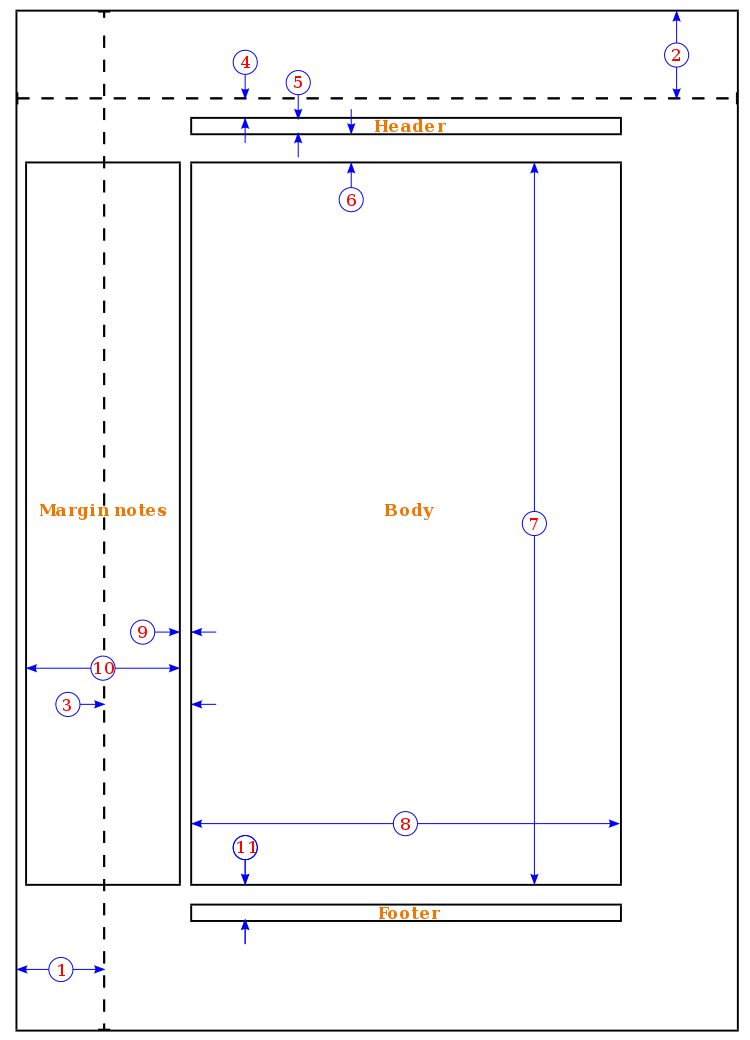
\includegraphics[width=\textwidth, height=\textheight, keepaspectratio]{images/Latex_layout.png}
		\end{columns}
	\end{frame}

	% crap
			%		\colorlet{circle area1}{blue!20}
			%		\colorlet{circle area2}{green!20}
 			%		\tikzset{
			%			% filled1/.style={fill=circle area1, draw=circle edge, thick},
			%			% filled2/.style={fill=circle area2, draw=circle edge, thick},
			%			filled/.style={fill=circle area, draw=circle edge, thick},
			%			outline/.style={draw=circle edge, thick}
			%		}
			%		% \only<4>{
			%		% 	\begin{tikzpicture}[thick, fill=blue!30]
			%		% 		\scope 
			%		% 			\clip (0,0) circle (2cm);
			%		% 			\fill (3,0) circle (2cm);
			%		% 		\endscope
			%		% 		\draw (0,0) circle (2cm) node {Matter};
			%		% 		\draw (3,0) circle (2cm) node {Form};
			%		% 	\end{tikzpicture}
			%		% }
			%		\only<4>{
			%			\begin{tikzpicture}
			%				\begin{scope}
			%					\clip \cirA;
			%					\draw[filled, even odd rule] \cirA
			%												 \cirB node {Form};
			%				\end{scope}
			%				\draw \cirA node {Matter}
			%							   \cirB;
			%			\end{tikzpicture}
			%		}
\end{document}
